\documentclass{IOS-Book-Article}     %[seceqn,secfloat,secthm]
\usepackage{mathptmx}
\usepackage{soul}\setuldepth{article}

%\normalfont
%\usepackage[T1]{fontenc}
%\usepackage{times}
%\usepackage[mtplusscr,mtbold]{mathtime}
\def\hb{\hbox to 11.5 cm{}}
%\usepackage[utf8]{inputenc}
%\usepackage[english]{babel}
\usepackage{graphicx}
\usepackage{float}
\usepackage{textcomp}
%\usepackage{xcolor}
\usepackage{booktabs}
\usepackage{tabulary}
\usepackage{tabularx}
\usepackage{csquotes}
\usepackage{siunitx}
\usepackage[disable]{todonotes}
%\usepackage{natbib} % does not seem to work with ios 1
\newcommand{\citet}{\cite}% citet is not defined without natbib
\newcommand{\citep}{\cite}% citep is not defined without natbib
\setlength{\marginparwidth}{2.1cm}% enough space for todonotes
\usepackage{listings}
\usepackage{aurl}
\daurl{ob}{http://www.snik.eu/ontology/bb/}
\daurl{bb}{http://www.snik.eu/ontology/bb/}
\daurl{meta}{http://www.snik.eu/ontology/meta/}
\lstset{language=SPARQL,breaklines=true}
\usepackage[noabbrev,capitalize]{cleveref}
\newcommand{\snikversion}{1.3.0}
\newcommand{\snikversionlink}{\href{https://github.com/snikproject/ontology/releases/tag/\snikversion}{\snikversion}}
\newcommand{\sniktriples}{\num{81499}}
% SELECT (COUNT(DISTINCT ?s) AS ?count) {?s a owl:Class. FILTER(STRSTARTS(STR(?s),"http://www.snik.eu/ontology/"))}
\newcommand{\snikclasses}{\num{4719}}
% SELECT (COUNT(DISTINCT ?s) AS ?roles) {?s meta:subTopClass meta:Role.}
\newcommand{\snikroles}{260}
% SELECT (COUNT(DISTINCT ?s) AS ?functions) {?s meta:subTopClass meta:Function.}
\newcommand{\snikfunctions}{\num{1310}}
% SELECT (COUNT(DISTINCT ?s) AS ?entiytypes) {?s meta:subTopClass meta:EntityTypes.}
\newcommand{\snikentitytypes}{\num{3182}}
% SELECT (COUNT(DISTINCT ?s) AS ?count) {{?s a rdf:Property.} UNION {?s a owl:ObjectProperty.} UNION {?s a owl:DataTypeProperty.} FILTER(STRSTARTS(STR(?s),"http://www.snik.eu/ontology/"))}
\newcommand{\snikproperties}{65}
%SELECT (COUNT(DISTINCT *) AS ?links) {?s ?p ?o. FILTER(STRSTARTS(STR(?o),"http://dbpedia")) }
\newcommand{\sniklinks}{579}

\begin{document}

\pagestyle{headings}
\def\thepage{}

\begin{frontmatter}              % The preamble begins here.


%\pretitle{Pretitle}
\title{SNIK Quiz: Automatic Generation of Multiple Choice Questionnaires about Information Management in Hospitals}
%\thanks{This work is supported by the DFG (German Research Foundation) under the Project SNIK, Grant no. 1605/7-1 and 1387/8-1.}%bug: will create an empty first page

\markboth{}{May 2022\hb}
%\subtitle{}

\author[A]{\fnms{Konrad} \snm{Höffner}%
%\thanks{Corresponding author: Konrad Höffner, Institute for Medical Informatics, Statistics and Epidemiology, Leipzig University,
\thanks{Corresponding author: Konrad Höffner, IMISE, Leipzig University,
Härtelstraße 16--18, 04107 Leipzig, Germany; E-mail: konrad.hoeffner@imise.uni-leipzig.de.}},
\author[A]{\fnms{Arne} \snm{Roszeitis}},
\author[A]{\fnms{Max Niclas} \snm{Wächtler}},
\author[A]{\fnms{Franziska} \snm{Jahn}},
\author[A]{\fnms{Alfred} \snm{Winter}}
\runningauthor{K. Höffner et al.}
%\address[A]{Institute for Medical Informatics, Statistics and Epidemiology (IMISE), Leipzig University, Germany}
%\address[A]{Institute for Medical Informatics, Statistics and Epidemiology, Leipzig University, Germany}
\address[A]{IMISE, Leipzig University, Germany}
%Medical Informatics, Management of Health Information Systemsi
%Härtelstraße 16--18, D-04107 Leipzig

\iffalse
\author{\IEEEauthorblockN{Konrad Höffner}
\IEEEauthorblockA{\textit{Institute for Medical Informatics, Statistics and Epidemiology} \\
\textit{Leipzig University}\\
Leipzig, Germany \\
\url{https://orcid.org/0000-0001-7358-3217}}
\and
\IEEEauthorblockN{Franziska Jahn}
\IEEEauthorblockA{\textit{Institute for Medical Informatics, Statistics and Epidemiology} \\
\textit{Leipzig University}\\
Leipzig, Germany \\
\url{https://orcid.org/0000-0002-7687-8544}}
\and
\and
\IEEEauthorblockN{Alfred Winter}
\IEEEauthorblockA{\textit{Institute for Medical Informatics, Statistics and Epidemiology} \\
\textit{Leipzig University}\\
Leipzig, Germany \\
%alfred.winter@imise.uni-leipzig.de}
\url{https://orcid.org/0000-0003-0179-954X}}
\and
\IEEEauthorblockN{Thomas Pause}
\IEEEauthorblockA{\textit{Institute for Medical Informatics, Statistics and Epidemiology} \\
\textit{Leipzig University}\\
Leipzig, Germany \\
\url{https://orcid.org/0000-0001-5832-4890}}
}
\fi
\begin{abstract}
%Textbooks contain abstract knowledge about a domain.
%Textbooks about information management in hospitals describe the planning, monitoring and directing of a hospital's information system.
SNIK is a knowledge base about the management of health information systems generated by extracting Linked Data from textbooks and other sources.
SNIK describes health information management functions, roles executing these functions, and entity types, the information used or updated by these functions.
%SNIK consists of the manually transformed content of three textbooks as Linked Open Data.
We present SNIK Quiz, a browser game in which students answer multiple-choice questions about information management in hospitals based on SNIK.
The questions are semi-automatically generated using several question templates in order to train basic facts, more complex patterns, and connections between textbooks encoded in SNIK.
%The data model describes information management functions, roles executing these functions and the information used or updated by these functions.

%SNIK provides applications that are used to teach students internationally.
%and the result of applying the data model to three textbooks, an interview and a standard.
%To compare, 
%, making it a natural fit for RDF, RDFS and OWL.
%As the domain is large and highly relevant to students of Medical Informatics, modelling the knowledge is not only possible but also very useful.
%We publish the result over several interfaces that are useful for researchers, administrators or students, depending on their objectives and capabilities.
\end{abstract}

% SWJ style
%\begin{keyword}
%\kwd{information management, information systems, hospital information management}
%\end{keyword}
% ICSCR style
%\begin{IEEEkeywords}
%linked open data, information management
%\end{IEEEkeywords}

% MIE style
\begin{keyword}
linked open data \sep information management \sep multiple choice quiz
\end{keyword}
\end{frontmatter}

\section{Introduction}
%A health information system (HIS) is the socio-technical subsystem of a care delivery organization~\citep{bb}.
%This includes its different application systems, computers, and network components as well as their users.
Medical informatics students, who are trained for executive positions in information management (IM) departments of healthcare institutions, such as hospitals, need a clear terminology of their domain.
This terminology is offered by SNIK~\citep{semantischesnetz,sniktec}, the Semantic Network of Information Management in Hospitals (\enquote{Krankenhaus} in German), which integrates knowledge extracted from three textbooks~\citep{bb,ob,he} and other sources such as interviews in the form of Linked Open Data.
In order to specify, which information should be extracted from the books and to facilitate comparisons, we use a common data model.
Because processed textbooks contain abstract knowledge instead of information about any specific hospital, all concepts are modelled as classes and instances simultaneusly, using OWL punning.
We thus call our data model the \enquote{meta model} in accordance with the term's definition as a shared modelling language~\citep[p.~8]{ob}.
The central entities of the meta model are enterprise functions, roles executing these functions, and entity types, the information used or updated by these functions, see \cref{fig:metamodel}.
%Because the textbooks describe those concepts in the abstract sense, and not those of any concrete hospital, those entities are modelled as classes and individuals at the same time, using OWL 2 DL punning.
%Thus, \emph{function}, \emph{role} and \emph{entity type} are metaclasses and the ontology of SNIK is a meta model as depicted in \cref{fig:metamodel}.
SNIK version \snikversionlink{} contains \sniktriples{} triples describing \snikproperties{} properties and \snikclasses{} classes, of which there are \snikroles{} roles, \snikfunctions{} functions and \snikentitytypes{} entity types.
%Applications include a graph visualization for exploratiory learning, 
%
\begin{figure}
\caption{The SNIK Quiz browser game available at \url{https://www.snik.eu/quiz}.}
\label{fig:snikquiz}
\centering
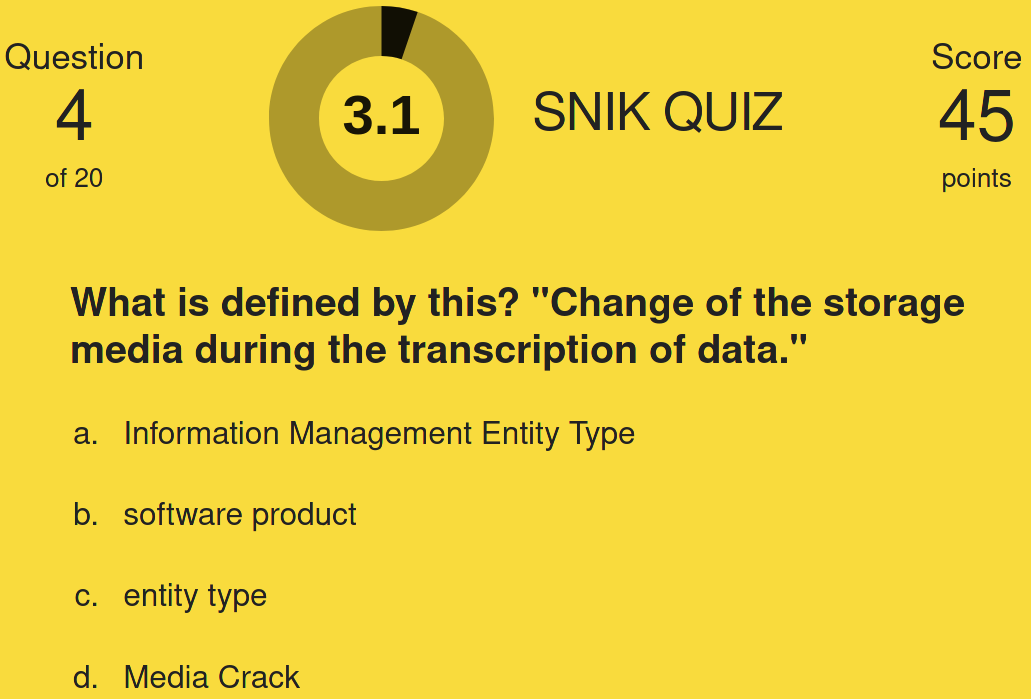
\includegraphics[width=0.6\textwidth]{img/snik-quiz.png}
\end{figure}
This paper presents SNIK Quiz, an open source\footnotemark{} browser game, see \cref{fig:snikquiz}, in which students answer multiple-choice questions about HIM, including an evaluation by domain experts and a student.
\footnotetext{Source code available under the MIT license at \url{https://github.com/snikproject/quiz}. The user interface is a fork of \url{https://github.com/davidrayoussef/react-quiz}.}
%A HIS processes data, information, and knowledge and its management involves planning, monitoring and directing those activities.
%Due to the complexity and the unique conditions in health care, HIS management is an challenging task.
%There are many different frameworks, textbooks and articles describing the scope of HIS management from the perspective of medical informatics.
%However, the disciplines of business informatics and information systems (IS) provide an even broader view on information systems and their management.
%A structured representation of the different perspectives leads to a holistic view on HIS management and helps help researchers and students connect their existing knowledge with further knowledge from other sources during research and learning.
%three textbooks~\citep{bb,ob,he} and other sources, see \cref{tab:source}.
%\section{Sources}\label{sec:sources}
%Three textbooks provide different views on the domain of Hospital Information Management:
%\citet{bb} presents a broad view on \enquote{typical architectures of health information systems and their systematic strategic management}.
%\citep{ob} concentrates on the \emph{tactical} management of information systems in general and on healthcare in particular.
%The focus of tactical management lies on the planning and operation of projects.
%\citet{he} explains information management beyond the scope of healthcare.
%Other sources are interviews and standards.
%CIOX is based on an interview with the CIO of the Universitätsklinikum Leipzig.
%IT4IT is based on the IT4IT standard.\todo{Sebastian: Was über Standards und IT4IT schreiben}
%
%We discuss advantages and disadvantages of the interfaces and give recommendations on which ones present the best compromise for different use cases and target audiences.
%We conclude with plans for future work on interlinking and visualization.
%As the domain is large and highly relevant to students of Medical Informatics, modelling the knowledge is not only possible but also very useful.
%Due to different frameworks and textbooks dealing with information management in healthcare, modelling the knowledge unravels the links between the different views on information management.
%These are only implicitly known or not known at all by experts in the field.
%
%
%Publishing textbook knowledge as Linked Data enables different ways of teaching.
%The data is continously revised: users constantly report wrong or missing data in the visualization, which is then corrected, respectively revised, by the researchers of the project.

\iffalse
\begin{table}[tbh]
\caption{The different ontologies and graphs of SNIK and their sources.
The namespace of each ontology is is equal to its URL with a slash suffix.
The graph group URL has no associated ontology and is the entry point of the RDF browser.
%All graphs are combined in the graph group \lowercase{\url{http://www.snik.eu/ontology}}.
}
\label{tab:source}
\begin{center}
%\begin{tabular}{\columnwidth}{lll}
\begin{tabular}{lll}
\toprule
\textbf{Prefix}	&\textbf{Ontology and Graph URL}			&\textbf{Source}\\		
\midrule
meta			&\url{http://www.snik.eu/ontology/meta}		&Meta Model\\
bb				&\url{http://www.snik.eu/ontology/bb}		&Textbook~\cite{bb}\\
ob				&\url{http://www.snik.eu/ontology/ob}		&Textbook~\cite{ob}\\
he				&\url{http://www.snik.eu/ontology/he}		&Textbook~\cite{he}\\
ciox			&\url{http://www.snik.eu/ontology/ciox}		&CIO Interview\\
it4it			&\url{http://www.snik.eu/ontology/it4it}	&Standard~\cite{it4it}\\
\midrule
sniko			&\url{http://www.snik.eu/ontology}			&Combined Graph Group\\
\bottomrule
\end{tabular}
\end{center}
\end{table}
\fi

\section{Methods}
\begin{figure*}
\caption{The SNIK meta model}
\label{fig:metamodel}
\centering
\includegraphics[width=\textwidth,trim={0 0 0 135mm},clip]{img/metamodel9s.pdf}
\end{figure*}
SNIK Quiz is designed as single-player game for English speaking students of Medical Informatics.
This group is diverse and includes students of Medicine, who may not have a background in Computer Science and Semantic Web technologies.
Target devices are PCs, tablets and smartphones, so multiple operating systems and input methods need to be supported.
Thus, SNIK Quiz is designed as an multiple choice quiz with at most four possible answers and published as an open source web application.
We employ an approach similar to Clover Quiz~\citep{cloverquiz}, which shows that Linked Data knowledge bases can be used to semi-automatically generate cross-domain multiple-choice questions on DBpedia~\citep{dbpedia}.
For each question (\emph{stem}), we generate a correct answer (\emph{key}) and one or more incorrect answers (\emph{distractors}).
The data is semi-automatically generated using SPARQL queries, such as \cref{lst:sparql}, on the public SPARQL endpoint of SNIK\footnote{\url{https://www.snik.eu/sparql}} followed by minimal postprocessing to achieve more natural looking questions.
The graph structure of SNIK allows the generation of difficult to guess distractors by using entities that are semantically close to the key, using path lengths of at most 2 in the graph.

\iffalse
\begin{figure}[h]
    \centering
    \includegraphics[width=0.5\columnwidth]{img/hierarchy.pdf}
    \caption{Excerpt of the SNIK class hierarchy. Source: \cite{snikposter}.}
	\label{fig:hierarchy}
\end{figure}
\vspace{-3pt}
\fi

%In order to specify, which information should be extracted from the books and to facilitate comparisons, we use a common data model.
%Because processed textbooks contain abstract knowledge instead of information about any specific hospital, all concepts are modelled as classes.
%We thus call our data model the \enquote{meta model} in accordance with the term's definition as a shared modelling language~\citep[p.~8]{ob}.
%The meta model (see \cref{fig:metamodel}) provides a common vocabulary for the domain of HIS management and thus defines, which superclasses and properties can be used.
%SNIK version \snikversionlink{} comprises five subontologies that are built upon the meta model, see Table 1.
%At the head of the class hierarchy (see \cref{fig:hierarchy}) is the \enquote{Top} class, which has exactly three disjunctive subclasses.
%At the head of the class hierarchy is the \enquote{Top} class, which has exactly three disjunctive subclasses.
%
%Following the meta model, each class has to be a subclass of exactly one of them.
%The correct superclass of a new concept can be found by answering the question: Who (\enquote{Role}) does what (\enquote{Function}) and which information (\enquote{EntityType}) is needed? If a concept is neither of them, it cannot be modeled using the meta model.
%As the subclass relation is transitive, a new class can be placed further down the hierarchy and it can still be inferred, whether it is a Function, Role or EntityType (see Figure 3).
%Besides the subclass relationship, two classes can be connected with relations provided by the meta model.
%The generic \enquote{is associated with} relationship carries little information.
%For example, a role and a function can be connected as \enquote{is involved in} \enquote{is responsible for} and \enquote{approves}.
%Relations that are neither of them can either be modeled by using the generic \enquote{is associated with} relation or by creating and using a new sub relation of \enquote{is associated with}
%
%As a concession to practicality, we express each geleral rule extracted from a textbook as a single triple using classes as subject and object, and a property of the meta model.
%For example, the rule "the CEO is involved in project reviews" is modelled as \enquote{\texttt{:Ceo} \aurl{meta}{isInvolvedIn} \texttt{:ProjectReview}.}, where \texttt{:Ceo} is a subclass of \aurl{meta}{Role} and \aurl{meta}{ProjectReview} is a subclass of \aurl{meta}{Function}.
%While an OWL restrictions using \aurl{owl}{someValuesFrom} and \aurl{owl}{allValuesFrom} would be technically correct, the knowledge is not expressed that specifically in the textbooks.
%Additionally, encoding each fact as a single triple facilitates tool support and prevents inconsistencies through non-atomic changes.

\section{Results}\label{sec:application}
The resulting question data is generated by several templates, as shown in \cref{tab:templates}, which are designed to either train basic facts, more complex patterns in one of the textbooks or connections between the different textbooks modelled in SNIK.

\begin{table}[h]
\caption{Quiz question templates with examples. When not otherwise noted, distractor entites are wrong answers that are neighbors of degree at most 2 of the correct answer.}%, with all being of the same type, see \cref{fig:metamodel}.}
\label{tab:templates}
\centering
\begin{tabulary}{\columnwidth}{lL}
\toprule
\textbf{Template}	&\textbf{Description}\\
\midrule
\textbf{Subject}		&Ask for the subject of a (subject, relation, object) triple given the relation and object.\\
%						&Distractors are labels of other classes (of the same type) that \emph{are not} related via the same relation to the same object but which are connected to the correct answer with a path of length at most 2.\\
Stem					&\emph{Who is responsible for Medical Admission?}\\
Key						&\emph{Physician}\\
Distractors				&\emph{Surgeon}, \emph{Health Care Professional}, \emph{Senior Physician}\\
\midrule
\textbf{Object}			&Ask for the object of a (subject, relation, object) triple given the subject and relation.\\
Stem					&\emph{The Specification Team is responsible for}$\ldots$\\
Key						&\emph{Functional Specification Document}\\
Distractors: 			&\emph{Project Team Member}, \emph{Sponsor}, \emph{Defining Project Organization}\\
\midrule
\textbf{Definition}		&Ask for the entity that fits the given textbook definition.\\
Stem					&\emph{What is defined by this? \enquote{X assures a defined quality of all processes and outcomes of the hospital}}\\
Key						&\emph{Internal Quality Management}\\
Distractors				&\emph{Activity}, \emph{Complaint}, \emph{Diagnosis}\\
\midrule
\textbf{Definitions}	&Present different definitions and ask, which of them fits the given entity.\\
Stem					&\emph{What defines the term Data Warehouse System?}\\
Key						&\emph{Application component that contains data which have been extracted from other application components, in order to support either hospital management or clinical research.}\\
Distractors				&\emph{Defines the hospital’s long-term strategic goals},
						\emph{An application component where the controlling rules for data processing are implemented as executable software},
						\emph{Summarizes monitored key performance indicators (KPIs) and compares them to the expected future state}\\
\midrule
\textbf{Intertwined}	&The correct answer and distractors are connected as shown in \cref{fig:intertwined}.\\
Stem					&\emph{In the context of Strategic Information Management, which one of the following triples belongs together the most?}\\
Key						&\emph{Chief Information Officer -- Department of Information management -- IM Staff}\\
Distractor 1			&\emph{Chief Information Officer -- Strategic Gap -- Corporate Strategy}\\
Distractor 2			&\emph{Chief Information Officer -- Ticket Evaluation -- Project Monitoring}\\
\midrule
\textbf{Occurence}		&Ask whether a given term is defined in one of the textbooks \cite{bb,ob}, both or neither~\citep{snikquizba}.\\
Stem					&\emph{In which contexts does the term \enquote{Health Insurance Company} occur?}\\
Key						&\emph{Strategic Information Management}\\
Distractors				&\emph{Tactical Information Management, Both Contexts, Neither}\\
\midrule
\textbf{CloseMatch}		&Transfer knowledge about one textbook~\citep{bb} to the other~\citep{ob} by confirming or denying statements about entity pairs that are marked as near equivalent~\citep{snikquizba}.\\
Stem					&\emph{In the Strategic Information Management, the Consultant is associated with the Long-Term HIS Planning, while in the Tactical Information Management, the Consultant is responsible for the Functional Specification Document.} (Key: True, Distractor: False)\\
%Key						&True\\
%Distractor				&False\\
\bottomrule
\end{tabulary}
\end{table}
%
\begin{lstlisting}[float, caption=SPARQL query generating the key and distractors for the \emph{definition} questions., label=lst:sparql,basicstyle=\ttfamily\footnotesize,frame=single]
SELECT SAMPLE(replace(str(?def),str(?cl),"X","i") as ?def) SAMPLE(str(?cl) as ?cl) SAMPLE(str(?a1l) as ?a1l) SAMPLE(str(?a2l) as ?a2l) SAMPLE(str(?a3l) as ?a3l) {
  ?class a owl:Class.
  ?class rdfs:label ?cl.
  FILTER(LANGMATCHES(LANG(?cl),"en"))
  ?class skos:definition ?def.
  FILTER(STRLEN(?def)>10&&STRLEN(?def)<600).
  FILTER(LANGMATCHES(LANG(?def),"en"))
  
  ?class (!(meta:subTopClass|rdf:type)){1,2} ?a1,?a2,?a3.
  owl:Class ^a ?a1,?a2,?a3.
  FILTER(?class!=?a1&&?class!=?a2&&?class!=?a3&&?a1<?a2&&?a2<?a3)

  ?a1 rdfs:label ?a1l. FILTER(LANGMATCHES(LANG(?a1l),"en"))
  ?a2 rdfs:label ?a2l. FILTER(LANGMATCHES(LANG(?a2l),"en"))
  ?a3 rdfs:label ?a3l. FILTER(LANGMATCHES(LANG(?a3l),"en"))
} GROUP BY ?class limit 1000
\end{lstlisting}
%
%Due to the limited nesting capabilties of SPARQL, which does not support loops but only subqueries that cannot access variables declared outside their scope, querying for distinct sets of 4 neighbours, where exactly one was connected over a certain property to a certain object, was not possible with our Virtuoso SPARQL endpoint initially.
%We circumvented the timeout by calculating the neighbour-relation as a first step and uploading it to the endpoint.
%
%SNIK Quiz is freely available as an open source web application.

%The definition approach focuses on the question of which definition is fitting for a given term. 
%To increase the difficulty of the strategy, the distractors are chosen to be at most two vertices away from the edge which represents the correct term, much like in the label-definition-type.

\begin{figure}
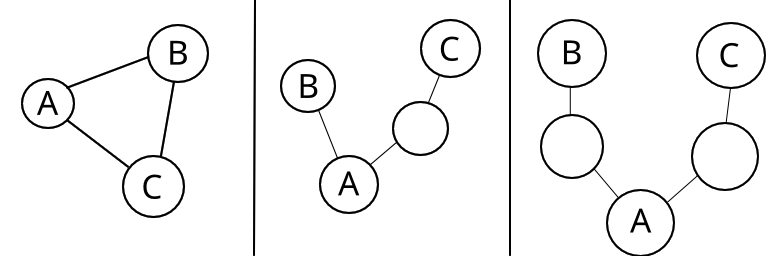
\includegraphics[width=0.7\textwidth]{img/intertwined_cml.png} 
\caption{Left to right: correct answer, difficult and easy distractor for the \emph{intertwined} question type~\citep{snikquizba}.}
\label{fig:intertwined}
\end{figure}

%This question type tests the connection between a textbook about tactical information management~\cite{ob} and one about strategic information management~\cite{bb} based on the existing \aurl{skos}{closeMatch} interlinks.
%The aim is to help students transfer knowledge about one textbook to the other.
%The questions have the form: \emph{\enquote{In [Tactical / Strategic IM], the [subject] [predicate] the [object], while in [Strategic / Tactical IM], the [subject] [predicate] the [object].}} with two possible answers: true and false.
%Examplarly questions are given in \cref{tab:closematch}.

%Dies beinhaltet dann Begriffe, welche in beiden Büchern auftreten. Ausgehend davon sollen dann ebenfalls in beiden Büchern auftretende Begriffe gesucht werden, welche verschiedene Grundklassen aufweisen: im einen Buch als Aufgabe und im anderen als Subjekt. Damit sollen dann Sätze gebildet werden, welche eine Gegenüberstellung in den Büchern erlauben, um so Brücken zu bauen und das Wissen des einen Buches effektiv auf das andere transferieren zu können. Ein Fragesatz könnte dann lauten: \enquote{In \textit{[Tactical / Strategic IM]}, the \textit{[Subjekt] [Prädikat]} the \textit{[Objekt]}, while in \textit{[Strategic / Tactical IM]}, the \textit{[Subjekt] [Prädikat]} the \textit{[Objekt]}} mit 2 Antwortmöglichkeiten, wahr und falsch.

\iffalse
\paragraph{occurence}
\begin{table}[h]
\begin{tabulary}{\textwidth}{LL}
\toprule
question	&correct\\
\midrule
In which contexts does the term \enquote{Automated Observation} occur?		&Tactical Information Management \\
In which contexts does the term \enquote{Health Insurance Company} occur?	&Strategic Information Management \\
In which contexts does the term \enquote{System Analysis} occur?			&Both Contexts \\
In which contexts does the term \enquote{System Administrator} occur?		&Neither\\
\bottomrule
\end{tabulary}
\caption{Exemplary \emph{occurrence}-questions and correct answers.}
\label{tab:occurence}
\end{table}

The \emph{occurence} question type is a specialization of \emph{closeMatch}, where the student has to choose whether a term occurs in~\cite{ob},~\cite{bb}, in both textbooks or neither of them.
Exemplary questions are given in \cref{tab:occurence}.
%mögliche Frage ist hier: \enquote{In which books does the term \emph{Chief Information Officer} occur?}.
The context of the questions can be augmented with the definitions of the concepts.
\fi



%The question types definition and subject were used to generate 1231 English questions, see \cref{tab:templates}.
The question types definition and subject were presented in a first prototype of SNIK Quiz to students of Medical Informatics from the Universities of Amsterdam, Heidelberg and Leipzig during the international Frank van Swieten lectures in 2019 and were positively received.
An extended version of SNIK Quiz including the query types definition, definitions, subject, intertwined, closeMatch and occurrence was rated by two experts of hospital information management and one student of Medical Informatics, see \cref{tab:eval}.
%The technical environment of SNIK is characterized in previous work [11].

\iffalse
\begin{table}[h]
\begin{tabularx}{\textwidth}{Xccc}
\toprule
Type				&rating interview 1	&rating interview 2	&rating interview 3\\
\midrule
label-definition	&3				&4				&3\\
definition-b		&4				&6				&3\\
contains-b			&5--6			&7				&6\\
\midrule
intertwined			&7				&7--8			&8\\
closeMatch			&8				&7--8			&8\\
occurence			&7				&5				&7\\
\bottomrule
\end{tabularx}
\caption{Rating given by interviewees based on the complexity of the questions on a scale between 1 and 10 with 10 representing maximum complexity.}
\label{tabelle:eval_komplex}
\end{table}
\fi

% transposed
\begin{table}[h]
\begin{tabularx}{\textwidth}{Xcccccc}
\toprule
			&definition		&definitions	&subject	&intertwined	&closeMatch	&occurence\\
\midrule
interview 1	&4					&3			&5--6		&7				&8			&7\\
interview 2	&6					&4			&7			&7--8			&7--8		&5\\
interview 3	&3					&3			&6			&8				&8			&7\\
\bottomrule
\end{tabularx}
\caption{Rating given by interviewees based on the subjective complexity of the questions on a scale between 1 and 10 with 10 representing maximum complexity~\citep{snikquizba}.}
\label{tab:eval}
\end{table}

\section{Discussion}
While the basic question types were received positively during the Frank van Swieten lectures and the evaluation ratings on subjective complexity show promising results, qualitative feedback on the more complex question types was mixed.
One of the experts questioned the didactic value of the \emph{intertwined} questions, as the users cannot know the exact graph structure of SNIK and thus may difficulties deciding, which triplets of concepts are most strongly connected.
While the closeMatch were rated as most complex, the complexity was seen mostly seen as grammatical and not enough on the didactically relevant relationships between the entities.
Contrary to the initial assumption that well explained questions would be beneficial, shorter questions were preferred as they could be read more quickly.

%However, only certain question types are feasible with SNIK.
%Because SNIK only contains the knowledge that the source textbooks describe, it does not contain the complete domain of Hospital Information Management.
%As such, negative questions are problematic, as the given relationship could hold in the real world but not be described in the textbook source of the class (open world assumption).
%The same problem concerns the distractors of positive questions.
%So this problem cannot be avoided.
%This is one of the reasons that we do not ask count questions like \enquote{How many functions is the CIO responsible for?}.
%Relationships could also hold implicitly through the subclass hierarchy.
%For example, \aurl{bb}{ChiefInformationOfficer} is a subclass of \aurl{bb}{InformationManagementStaff}, which is responsible for \aurl{bb}{OperationalInformationManagement}.
%It is unclear, whether the CIO is also responsible for operational information management.
%systematic review of multiple choice question generation from ontologies
%complex questions, 
%\cite{ontologybasedmultiplechoice}

%\cref{tab:templates} subclasses and superclasses
%because of OWL punning entities are individuals but also classes and can have superclasses and subclasses
%subclasses of the correct answer are semantically correct because subclasses are subsets
%superclasses on the other hand are only partially correct because the relation only holds for the subclass
%example who is responsible for medical admission: Health Care Professional - Physician - Senior Physician
%however SPARQL endpoint doesnt do inferencing so it will not mark that as correct
%we could add the transitive hull for such triples but we think it is good like this, it increases the difficulty and you need to choose the most general correct answer


%It can be combined with other knowledge in biomedical and health informatics and in other disciplines.

%\section{Future Work}
\section{Conclusions}
SNIK Quiz shows that knowledge on the management of information systems in medicine and health care can be used to semi-automatically generate multiple-choice questions.
While preliminary evaluations show promising results, the complex question types need to be investigated further.
Future work should also include a quantitative evaluation of learning efficiency when supplementing courses with SNIK Quiz.
%Use of neural networks and language models in combination with linked data to generate more natural questions and answers is another avenue for further exploration.

%\section{Acknowledgments}
%This work is supported by the DFG (German Research Foundation) under the Projects SNIK, grant no. 1605/7-1 and 1387/8-1, as well as HITO, grant no. WI 1605/11-1 and I3726-N31.
%We thank the publishers ... and ... for granting us permission to publish the subontologies based on the textbooks \citet{bb,ob,he} under an open license.
%\nocite{*} 
%\bibliographystyle{ios1}
\bibliographystyle{vancouver}
\bibliography{paper,snik,relatedwork}
\end{document}
